\documentclass[conference]{IEEEtran}
\IEEEoverridecommandlockouts

\usepackage{cite}
\usepackage{amsmath,amssymb,amsfonts}
\usepackage{graphicx}
\usepackage{textcomp}
\usepackage{xcolor}
\usepackage{booktabs}
\usepackage{url}
\graphicspath{{clarkson2_30day_model/figures/}}

\begin{document}

\title{AWARe: Adapting Behavioral Biometric Authentication to Longitudinal Keystroke Drift}

\author{
\IEEEauthorblockN{Keyaba Gohil, Sai Akshitha Boddupalli}
\IEEEauthorblockA{
\textit{Department of Computer Science}\\
\textit{San Jose State University}\\
San Jose, CA, USA
}
}

\maketitle

% ============================================================
% ABSTRACT
% ============================================================

\begin{abstract}
Keystroke-dynamics authentication relies on behavioral patterns that may change over time, causing an enrollment model to become less representative of a legitimate user. AWARe investigates longitudinal behavioral drift in keystroke-based biometric authentication and whether targeted model adaptation can recover genuine-user performance without compromising impostor rejection. Using the Clarkson II longitudinal keystroke dataset, we train a two-layer Transformer encoder on users' initial 30-day activity and evaluate its frozen 32-dimensional embedding representation on chronologically later behavior. The first-30-day test EER is 13.98\%, while EER increases to 25.55\%, 26.65\%, and 24.94\% in later Stages 1--3, respectively. We quantify user-specific embedding drift, use causal tracing to localize recoverable internal representations, and evaluate ROME-inspired rank-one editing. Causal tracing recovers 88.8\% of the target user's embedding-distance degradation at Transformer layer 2. Controlled editing experiments show that stronger edits reduce genuine-user FRR but also increase FAR; at 20 optimization steps, Stage 2 FRR improves by 6.07 percentage points while FAR increases by 4.25 points. Thus, representation recovery is possible, but the current editing configuration does not satisfy the predefined security constraints.
\end{abstract}

\begin{IEEEkeywords}
behavioral biometrics, keystroke dynamics, continuous authentication, behavioral drift, Transformer, causal tracing, model editing
\end{IEEEkeywords}


% ============================================================
\section{Problem Statement and Motivation}
% ============================================================

Keystroke dynamics is a behavioral biometric that authenticates users from temporal patterns in their typing~\cite{subash,morales}. Unlike physiological biometrics, behavioral characteristics are not necessarily stationary. Typing rhythm may change with device familiarity, environment, physical state, or natural behavioral variation. A biometric model trained during enrollment may therefore become progressively less representative of the same legitimate user.

This project investigates \textbf{longitudinal behavioral drift in keystroke-based biometric authentication}. We ask whether a model trained using a user's initial activity continues to recognize that user when evaluated on chronologically later typing. Our hypothesis is that later genuine samples can move farther from the enrollment representation, cross a fixed authentication threshold, and increase false rejection rate (FRR).

This creates a security--usability trade-off. A static model may increasingly reject legitimate users, but unrestricted adaptation may reduce security if an update that accommodates a genuine user also increases acceptance of impostors. A useful adaptation mechanism must therefore reduce drift-induced rejection while preserving false acceptance rate (FAR).

This matters directly for continuous authentication: a false rejection can interrupt an authorized user's session, while an overly permissive update can create an avenue for impostor acceptance.

AWARe first establishes a frozen enrollment-time baseline, then measures longitudinal embedding drift, uses causal tracing to localize recoverable representations, and finally evaluates whether a ROME-inspired rank-one edit can provide targeted adaptation while satisfying explicit FRR and FAR constraints. This adaptation focus follows prior work on template updating and long-term user frustration in continuous authentication~\cite{mhenni,huh}.

\textbf{Nature of Project:} Build a robust keystroke biometric authentication system capable of adapting to longitudinal behavioral drift while preserving impostor rejection.\\
\textcolor{blue}{Scope change since the proposal: the revised checkpoint adds causal tracing and ROME-inspired rank-one editing as targeted adaptation analyses.}


% ============================================================
\section{Data Engineering}
% ============================================================

\subsection{Dataset Origin and Characteristics}

The project uses the \textbf{Clarkson II Keystroke Dataset}, a longitudinal free-text keystroke dataset distributed by Clarkson University~\cite{clarkson}. Unlike fixed-password datasets, Clarkson II records naturally occurring keyboard activity over extended periods, making it particularly useful for studying behavioral biometric template aging and longitudinal drift. The data are distributed as raw keyboard-event logs rather than precomputed biometric feature vectors. Each event records temporal information, a press/release event type, and key information, allowing hold and inter-key timing features to be reconstructed.

For this project, the available local release contains \textbf{100 user files and 25,261,528 raw keyboard events}. User identity is provided by the source file and serves as the ground-truth subject label. Authentication labels such as genuine and impostor are not explicitly stored in the raw dataset; they are constructed during verification by comparing a query with the claimed user's enrollment prototype.

Because Clarkson II records asynchronous keyboard events rather than regularly sampled signals, a fixed sampling frequency is not applicable.

\begin{table}[htbp]
\caption{Dataset characteristics and chronological coverage.}
\label{tab:data}
\centering
\scriptsize
\begin{tabular}{p{0.34\columnwidth}p{0.57\columnwidth}}
\toprule
\textbf{Quantity} & \textbf{Observed value}\\
\midrule
Raw subjects/files & 100 user files; 25,261,528 raw events\\
Event schema & Timestamp, press/release indicator, key code\\
Labels & File identity; genuine/impostor labels generated during verification\\
Validated raw events & 25,261,511 passed; 17 malformed rows skipped\\
Valid pairs/windows & 5,498,480 valid pairs; 41,895 first-30-day windows\\
Initial coverage & 89 users with at least one usable window; 85 with at least three\\
Later coverage & 37,391 windows from 82 users across Stages 1--3\\
Stage coverage & S1: 17,145/73 users; S2: 11,986/56; S3: 8,260/68\\
\bottomrule
\end{tabular}
\end{table}

The dataset is accessed from the Clarkson II distribution maintained by Clarkson University's Center for Identification Technology Research (CITeR)~\cite{clarkson}. It is not distributed under an unrestricted public license: CITeR instructs researchers to request the dataset by contacting \texttt{dhou@clarkson.edu} and identifying the specific release; access is provided after completing an agreement with the dataset authors. We therefore do not redistribute the raw data or commit it to GitHub. Users must obtain the data directly from the provider and place the extracted files in the repository's \texttt{filtered\_dataset/} directory before running preprocessing.

The longitudinal free-text setting is valuable for this project because it captures natural temporal variation, but it also introduces limitations. Users contribute highly unequal amounts of activity, recording durations differ substantially, and raw event logs contain logger and event-pairing anomalies. Furthermore, the dataset does not provide an externally defined ``drift'' label; drift must be operationally measured from changes in the learned biometric representation.

\subsection{Schema Sanity and Cleaning}

Of the 25,261,528 raw events, \textbf{25,261,511 passed initial schema validation}; 17 malformed rows were skipped. Initial quality analysis found \textbf{21 timestamp backsteps}, 870,748 equal-timestamp events, and 395,335 consecutive duplicate rows.

An initial press/release pairing pass produced 134,225 negative hold-time pairs across seven users. Splitting event streams at timestamp backsteps and resetting the pairing queues eliminated these negative durations.

A separate long-hold problem remained. Before thresholding, 10,425,149 nonnegative press/release pairs were available. The approximate median hold time was 2.12~s, whereas the 75th percentile was approximately 136,269~s, and more than 3.8 million pairs exceeded 300~s. Such durations are inconsistent with ordinary key holds and indicate missing releases, logger behavior, or incorrect event pairing.

We compared maximum hold thresholds of 5, 10, and 30~s, which retained 52.74\%, 54.78\%, and 57.67\% of candidate pairs, respectively. A \textbf{5-s threshold} was fixed for all checkpoint experiments, retaining \textbf{5,498,480 valid pairs} and removing 4,926,669 long-hold pairs.

\subsection{Feature Engineering}

Cleaned events are segmented into non-overlapping windows of \textbf{50 press/release pairs} with stride 50. Four timing features are retained for each pair: hold time, press-to-press time, release-to-press time, and inter-event time.

Although key identity exists in the raw logs, it is intentionally excluded from model input. Authentication therefore depends on \textit{how} a user types rather than the textual content typed.

Each timing value is transformed as

\begin{equation}
x'=\log(1+\max(x,0)),
\label{eq:transform}
\end{equation}

then standardized using means and standard deviations estimated \textbf{only from the first-30-day training split}. The resulting model input has shape $50\times4$. The same training statistics are reused for every later stage to prevent temporal leakage.

\subsection{Chronological Split}

For each user, activity from the first timestamp through the following 30 days forms the initial model-development period. This subset contains \textbf{2,563,906 valid event pairs and 41,895 windows}. Of the 100 source users, 89 produce at least one usable window and 85 produce at least three.

All usable activity after day 30 is retained for longitudinal evaluation. For each user independently, the remaining observation interval is divided chronologically into three equal temporal intervals:

\begin{itemize}
    \item \textbf{Stage 1}: earliest later behavior, used for drift ranking and adaptation;
    \item \textbf{Stage 2}: middle behavior, used as the primary held-out evaluation;
    \item \textbf{Stage 3}: latest behavior, used as secondary held-out evaluation.
\end{itemize}

The later-stage data contain \textbf{37,391 windows from 82 users}: 17,145 Stage 1 windows from 73 users, 11,986 Stage 2 windows from 56 users, and 8,260 Stage 3 windows from 68 users. Median observed stage durations are 43.4, 42.2, and 32.7 days, respectively. The median remaining observation span after day 30 is 193.9 days, with a maximum of 1,104.9 days.


% ============================================================
\section{Exploratory Data Analysis}
% ============================================================

\subsection{Univariate Analysis and Data Quality}

Univariate analysis of hold duration revealed an extreme long-tailed distribution. The contrast between the 2.12-s median and approximately 136,269-s 75th percentile demonstrated that the raw event pairing could not be treated as ordinary typing without quality filtering.

Fig.~\ref{fig:hold_dist} shows the resulting window-level hold-time distribution. The clipped histogram makes the ordinary typing mass visible while the accompanying boxplot confirms the strong right-tail behavior.

\begin{figure}[htbp]
    \centering
    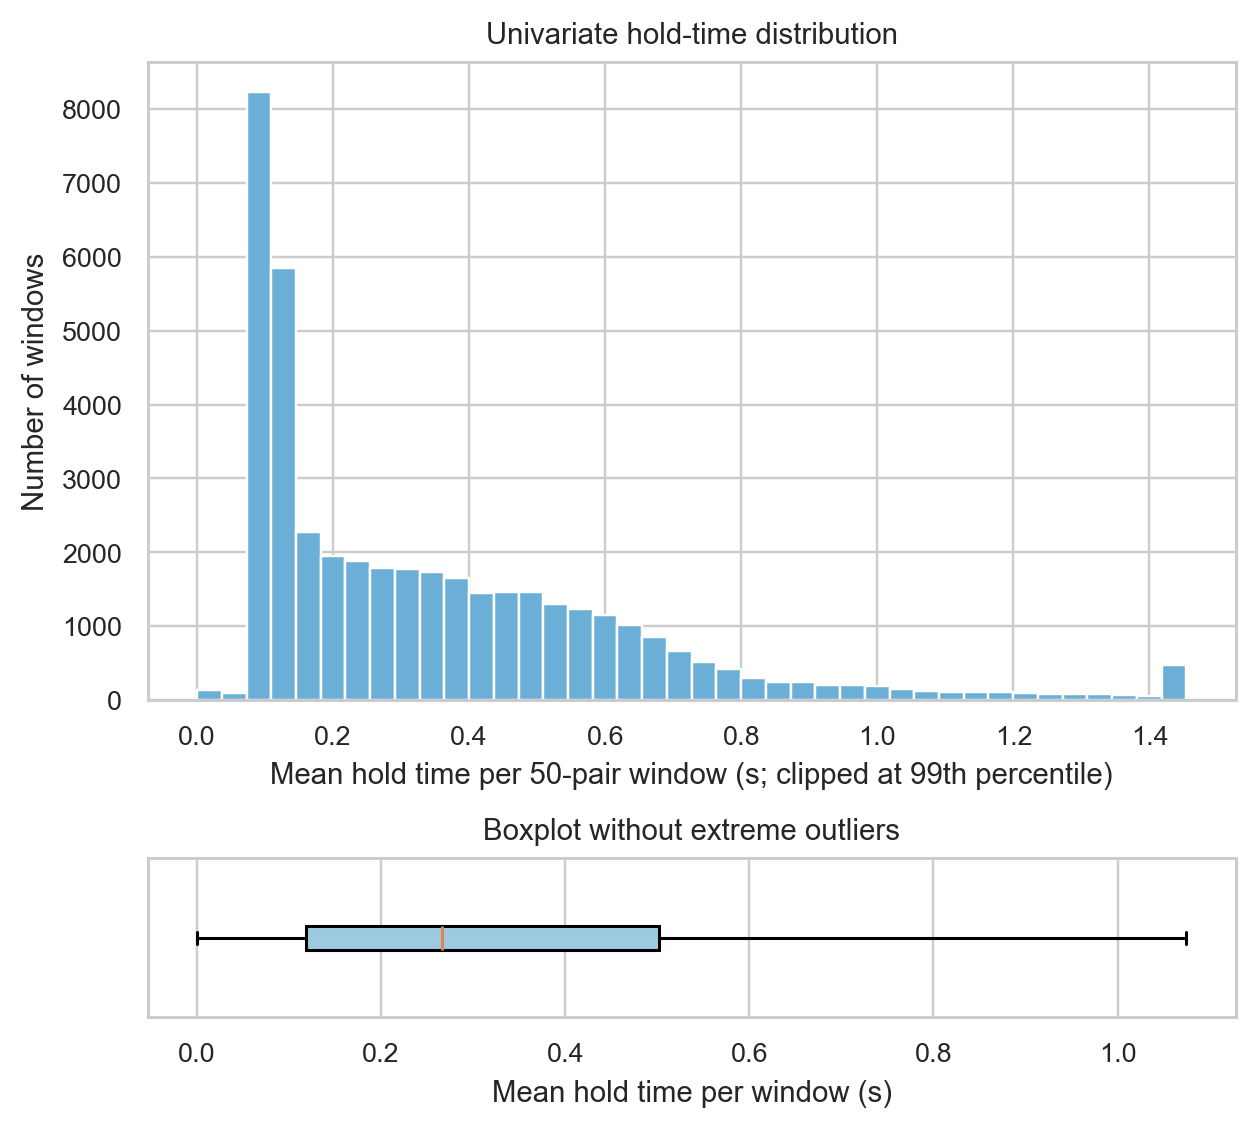
\includegraphics[width=\columnwidth]{hold_time_distribution.png}
    \caption{Univariate distribution of mean hold time per 50-pair window. The clipped histogram shows the central mass, while the boxplot summarizes spread without allowing extreme outliers to dominate the axes.}
    \label{fig:hold_dist}
\end{figure}

Threshold sensitivity analysis showed that increasing the maximum allowed hold duration from 5 to 30~s retained only an additional 4.93\% of candidate pairs while admitting substantially longer and behaviorally questionable holds. Fig.~\ref{fig:hold} therefore supports the fixed 5-s preprocessing threshold.

\begin{figure}[htbp]
    \centering
    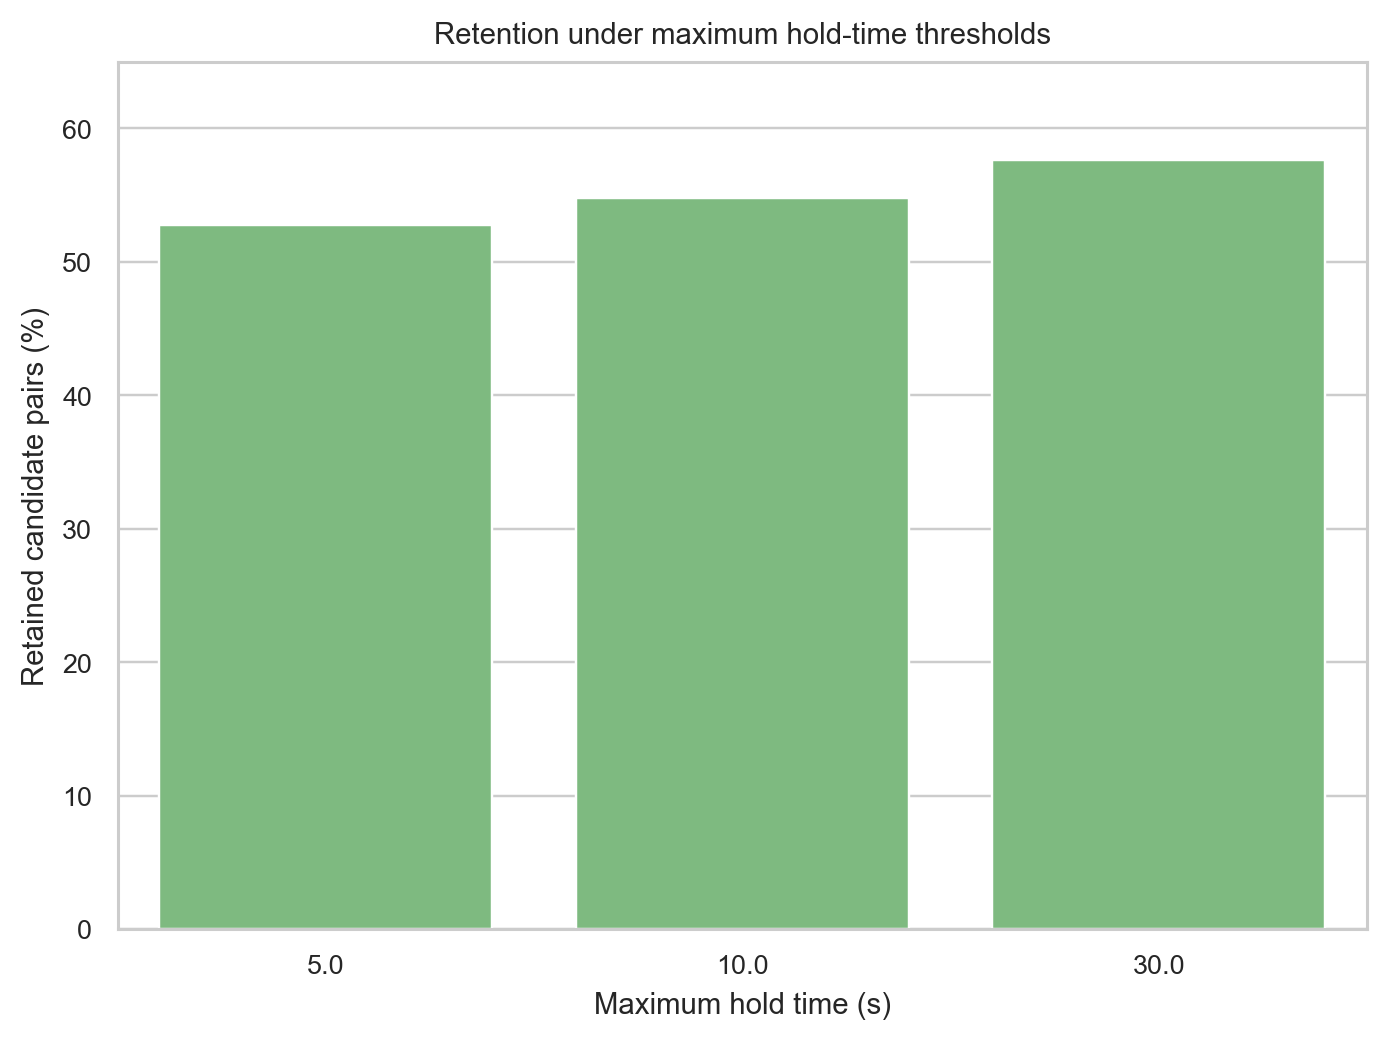
\includegraphics[width=\columnwidth]{01_threshold_retention.png}
    \caption{Retention of valid press/release pairs under different maximum hold-time thresholds. The 5-s operating point retains 52.74\% of candidate pairs while excluding implausibly long holds.}
    \label{fig:hold}
\end{figure}


\subsection{Bivariate Feature Analysis}

Relationships among the four timing features are evaluated using pairwise correlation analysis. This analysis is intended to identify strongly related timing measurements and determine whether multiple features encode overlapping temporal information.

The cleaned window table contains no valid release-to-press values, so correlations involving that feature are reported as ``N/A'' rather than treated as zero. This missingness is itself a documented data-quality result.

\begin{figure}[htbp]
    \centering
    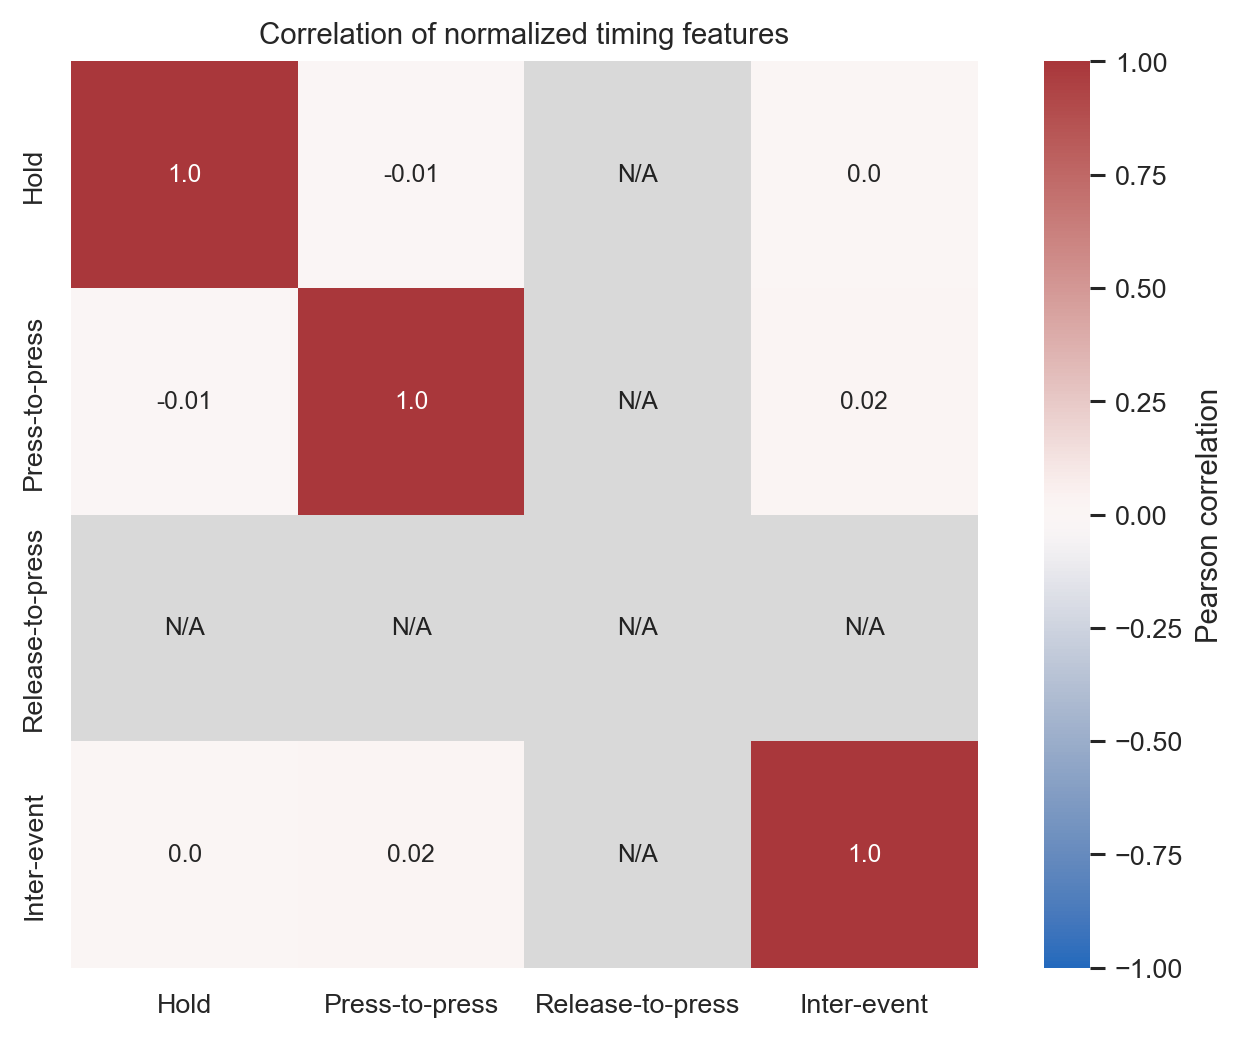
\includegraphics[width=\columnwidth]{feature_correlation_matrix.png}
    \caption{Pairwise Pearson correlation among the four normalized timing features. Gray ``N/A'' cells indicate that release-to-press had no valid values after cleaning, rather than implying zero correlation.}
    \label{fig:corr}
\end{figure}


\subsection{Class Balance and User Coverage}

The biometric classes correspond to user identities. The source data are not balanced: users contribute different numbers of valid windows, and user availability also changes across longitudinal stages. The first-30-day model contains usable windows from 89 users, whereas only 73, 56, and 68 users contribute windows to Stages 1, 2, and 3, respectively. Fig.~\ref{fig:balance} visualizes these four distributions directly.

This imbalance motivates reporting verification metrics such as FAR, FRR, and EER rather than relying only on overall classification accuracy. Longitudinal analyses also impose minimum-window eligibility requirements so that conclusions are not based on users with only a few observations.

\begin{figure}[htbp]
    \centering
    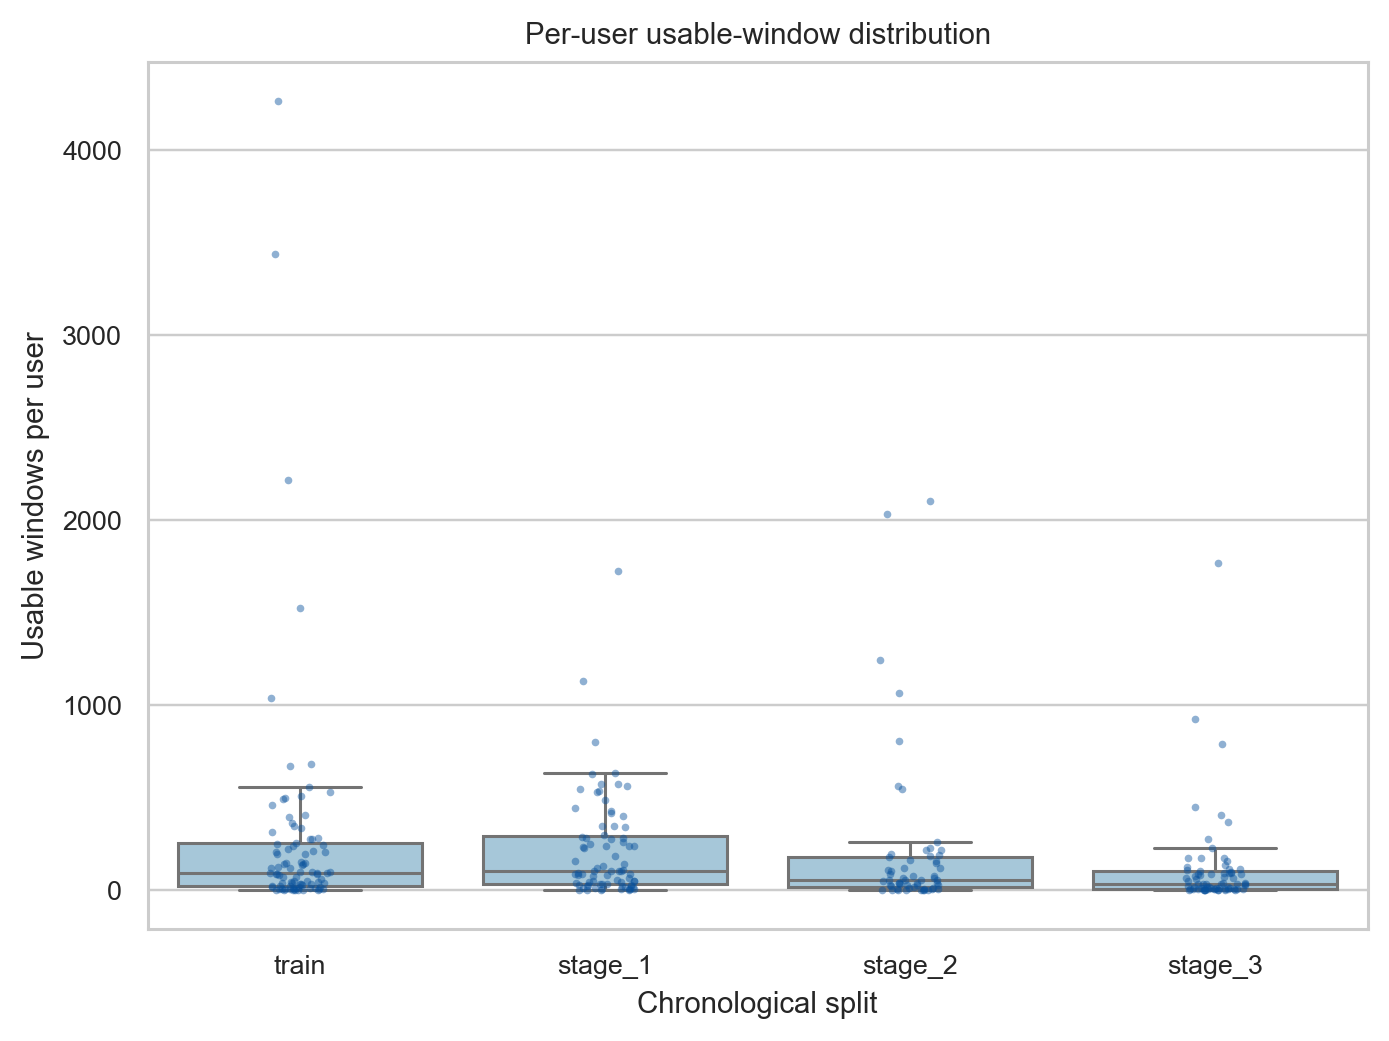
\includegraphics[width=\columnwidth]{user_window_distribution.png}
    \caption{Distribution of usable sequence windows across users in the first-30-day training split and later longitudinal stages. Unequal activity and changing user coverage motivate minimum-window eligibility criteria and per-rate biometric evaluation.}
    \label{fig:balance}
\end{figure}


\subsection{Longitudinal Embedding Drift}

After training, each first-30-day training window is converted into a normalized 32-dimensional embedding. For user $u$, the enrollment prototype is

\begin{equation}
p_u=\frac{1}{N_u}\sum_{i=1}^{N_u}f(x_i).
\label{eq:prototype}
\end{equation}

Verification uses Euclidean distance

\begin{equation}
d(z,p_u)=\|z-p_u\|_2.
\label{eq:distance}
\end{equation}

For each user, absolute longitudinal drift at stage $s$ is

\begin{equation}
D_{u,s}=\bar d_{u,s}-\bar d_{u,\mathrm{test}}.
\label{eq:drift}
\end{equation}

Positive values indicate movement away from the enrollment representation.

Users are included in drift ranking only when a stage contains at least five windows. The saved analysis ranks \textbf{74 users}. User \texttt{163748} exhibits the largest mean absolute drift at \textbf{+0.7299}, corresponding to approximately \textbf{+236.8\% relative drift}. Its Stage 2 and Stage 3 increases are +0.8672 and +0.8223, respectively.

Fig.~\ref{fig:drift} shows that longitudinal degradation is strongly user dependent rather than uniform across the population.

\begin{figure}[htbp]
    \centering
    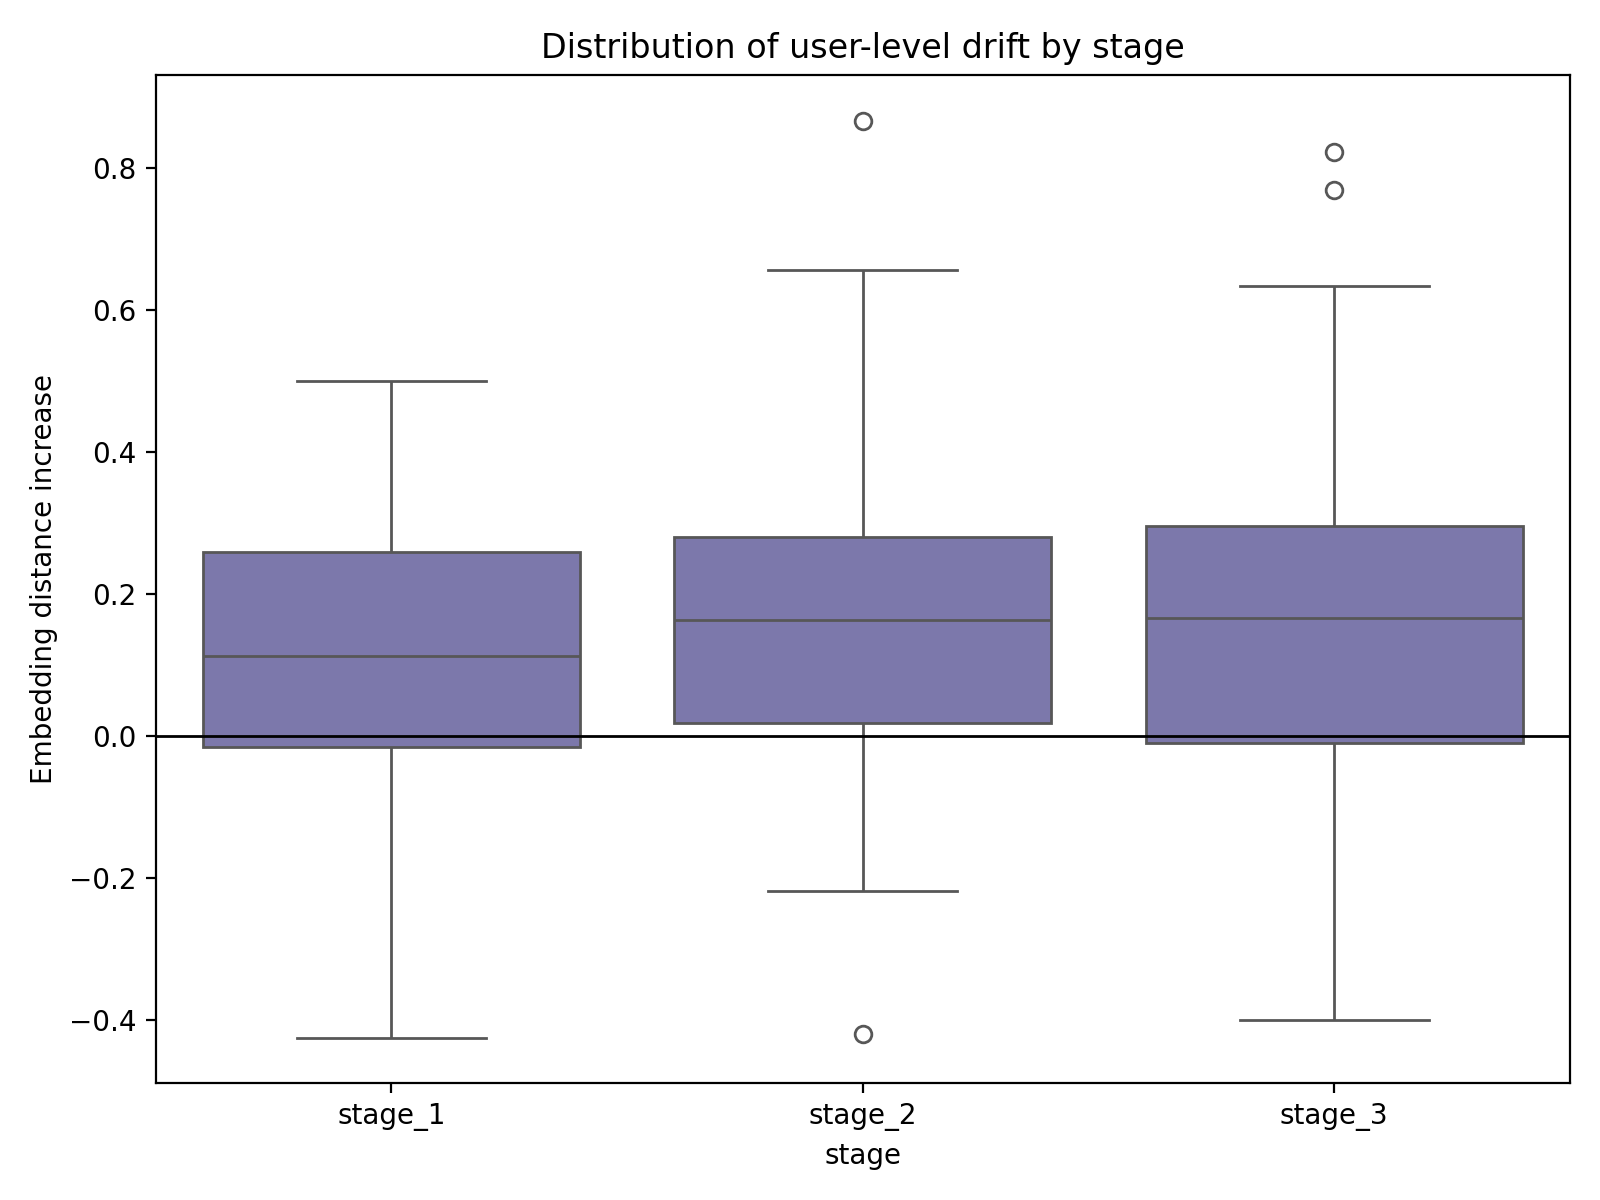
\includegraphics[width=\columnwidth]{user_drift_by_stage_boxplot.png}
    \caption{Distribution of user-level absolute embedding drift across later stages. Positive values indicate movement away from the original enrollment representation.}
    \label{fig:drift}
\end{figure}


% ============================================================
\section{Baseline Implementation and Preliminary Results}
% ============================================================

\subsection{Baseline Model and Verification Protocol}

The authentication backbone is a Transformer encoder. Each $50\times4$ sequence is projected to $d_{\mathrm{model}}=64$, combined with learned positional embeddings, and processed by \textbf{two Transformer encoder layers with four attention heads}. Mean pooling across the 50 events produces a sequence representation that is projected to a \textbf{32-dimensional normalized embedding}. This sequence-modeling choice is consistent with prior free-text continuous-authentication systems using neural sequence models~\cite{lin}.

During training, the network is optimized as an \textbf{89-user classification model}. The classification objective learns discriminative user representations; verification subsequently uses the normalized embeddings rather than classifier logits.

The best checkpoint was selected at \textbf{epoch 32} using adaptation-set EER with early stopping. A query is accepted when

\begin{equation}
d(z,p_u)\leq\tau,
\end{equation}

where the fixed operating threshold is

\begin{equation}
\tau\approx1.1886.
\end{equation}

The threshold is selected from the initial verification sweep at the operating point where FAR and FRR are approximately equal. We freeze this point before longitudinal evaluation so that later stages measure genuine temporal degradation rather than threshold recalibration.

The best model achieves \textbf{13.70\% EER} on the adaptation split and \textbf{13.98\% EER} on the first-30-day test split. At the fixed operating point, the test split contains \textbf{8,368 genuine trials} and \textbf{33,768 impostor trials}; FRR is \textbf{1,171/8,368 = 13.99\%} and FAR is \textbf{4,717/33,768 = 13.97\%}.

For genuine trials $G$ and impostor trials $I$,

\begin{equation}
\mathrm{FRR}=
\frac{\#\{g\in G:d_g>\tau\}}{|G|},
\end{equation}

\begin{equation}
\mathrm{FAR}=
\frac{\#\{i\in I:d_i\leq\tau\}}{|I|}.
\end{equation}

The corresponding adaptation split contains 8,255 genuine and 32,508 impostor trials; its fixed-threshold errors are 1,132 false rejects and 4,447 false accepts. These integer counts are reported alongside every rate to make the denominators explicit.


\subsection{Longitudinal Baseline Results and Error Analysis}

The same frozen model, enrollment prototypes, and threshold $\tau=1.1886$ are evaluated on chronologically later behavior.

\begin{table}[htbp]
\caption{Frozen-Model Longitudinal Performance}
\label{tab:longitudinal}
\centering
\scriptsize
\begin{tabular}{lccc}
\toprule
\textbf{Period} & \textbf{EER} & \textbf{FAR (FA/Imp.)} & \textbf{FRR (FR/Gen.)}\\
\midrule
30-day test & 13.98\% & \shortstack{13.97\%\\(4,717/33,768)} & \shortstack{13.99\%\\(1,171/8,368)}\\
Stage 1 & 25.55\% & \shortstack{25.52\%\\(381,718/1,496,000)} & \shortstack{25.58\%\\(4,349/17,000)}\\
Stage 2 & 26.65\% & \shortstack{26.70\%\\(281,588/1,054,504)} & \shortstack{26.60\%\\(3,188/11,983)}\\
Stage 3 & 24.94\% & \shortstack{24.92\%\\(178,577/716,584)} & \shortstack{24.97\%\\(2,033/8,143)}\\
\bottomrule
\end{tabular}
\end{table}

Stage 2 exhibits the largest EER, increasing by \textbf{12.67 percentage points} relative to the initial test period. All three later stages remain near 25--27\% EER compared with 13.98\% during the first-30-day test.

The primary baseline failure mode is therefore \textbf{longitudinal genuine-user drift}: later genuine embeddings move farther from their fixed enrollment prototype and increasingly cross the original authentication threshold. The fact that error rates remain elevated across all three later stages suggests that the degradation is not a single isolated temporal anomaly.

Figure~\ref{fig:drift-metrics} visualizes this result directly: EER rises from 13.98\% in the first-30-day test to 25.55\%, 26.65\%, and 24.94\% in Stages~1--3, while the fixed-threshold FAR and FRR show the same degradation pattern. The increase in FRR indicates greater legitimate-user rejection as later genuine embeddings move away from enrollment. The simultaneous FAR increase indicates that the later score distributions also admit more impostor trials, so simply loosening the threshold would not solve the drift problem.

\begin{figure}[t]
\centering
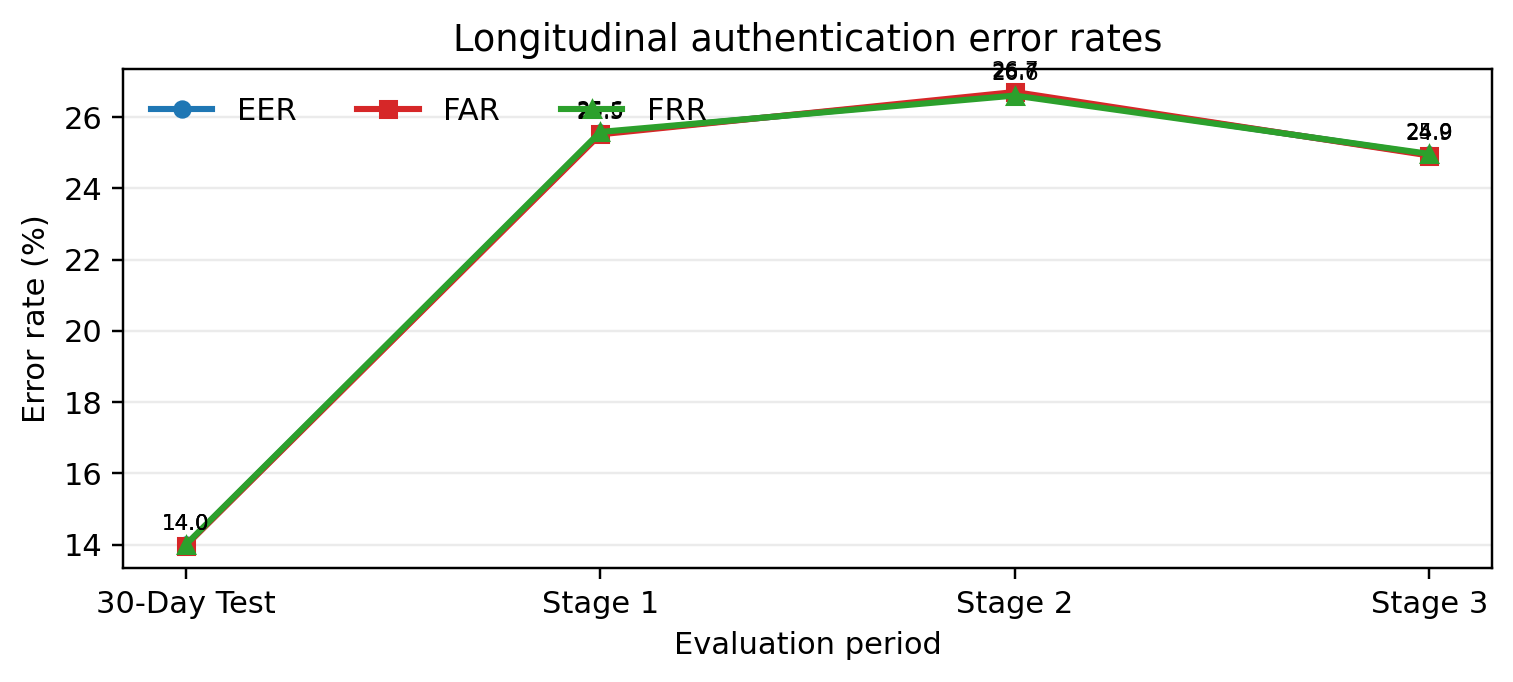
\includegraphics[width=\columnwidth]{longitudinal_drift_metrics.png}
\caption{EER, FAR, and FRR across the first-30-day test and later evaluation stages. The sustained increase after enrollment provides direct evidence of longitudinal drift.}
\label{fig:drift-metrics}
\end{figure}

For each period, EER is computed by sweeping the threshold over the saved genuine and impostor scores and selecting the point where FAR and FRR are closest. FAR and FRR in the table and figure are reported at the fixed enrollment threshold $\tau=1.1886$; therefore, EER summarizes separability while fixed-threshold FAR/FRR quantify deployment risk.


\subsection{Causal Tracing}

Causal tracing is performed on the highest-drift user, \texttt{163748}, using Stage 2 windows. The unpatched Stage 2 mean distance from this user's enrollment prototype is \textbf{1.1755}. At each intervention point, the activation is replaced with the corresponding mean activation obtained from the same user's first-30-day training windows. User \texttt{118630} serves as a wrong-user control.

\begin{table}[htbp]
\caption{Causal Tracing for User 163748}
\label{tab:causal}
\centering
\begin{tabular}{lcc}
\toprule
\textbf{Intervention} & \textbf{Patched Dist.} & \textbf{Recovery}\\
\midrule
Input projection & 0.9548 & 18.8\%\\
Transformer layer 1 & 0.1669 & 85.8\%\\
Transformer layer 2 & 0.1311 & 88.8\%\\
Post-encoder norm. & 0.1229 & 89.5\%\\
Embedding projection & 0.1224 & 89.6\%\\
\bottomrule
\end{tabular}
\end{table}

Transformer layer 2 is selected as the meaningful editable internal location: patching it reduces mean distance from 1.1755 to 0.1311 and recovers \textbf{88.8\%} of the observed degradation. Later normalization/projection interventions achieve slightly higher numerical recovery but do not represent comparable internal storage locations. The wrong-user control does not show the same consistent recovery.


\subsection{ROME-Style Rank-One Adaptation}

The ROME-style edit therefore targets the second Transformer layer's feed-forward \texttt{linear2} projection, following the localized feed-forward editing motivation of ROME~\cite{rome}. For each target user, a key vector $k$ is computed from mean Stage 1 activations, while covariance $C$ is estimated from first-30-day training windows. A desired value vector $v$ is optimized while the original model remains frozen, with a replay buffer used to preserve previously learned behavior.

The final update is

\begin{equation}
W_{\mathrm{new}}=
W+
\frac{(v-(Wk+b))(C^{-1}k)^T}
{(C^{-1}k)^Tk}.
\label{eq:rome}
\end{equation}

Each update has measured rank 1. The original prototypes and $\tau=1.1886$ threshold remain fixed after editing.

An edit succeeds only if Stage 2 FRR decreases by at least 5 percentage points, Stage 3 FRR does not increase, FAR increases by no more than 1 point, first-30-day test FRR increases by no more than 2 points, and the update remains rank 1.


\subsection{Controlled Edit-Strength Results}

Five Stage-1-ranked users (\texttt{163748}, \texttt{132109}, \texttt{562519}, \texttt{756382}, and \texttt{748549}) are evaluated with $v_{\mathrm{steps}}\in\{1,5,20\}$. Adaptation and replay sizes remain fixed at 64 windows each.

\begin{table}[htbp]
\caption{Controlled ROME Edit-Strength Results}
\label{tab:rome}
\centering
\begin{tabular}{lccc}
\toprule
\textbf{$v$ steps} & \textbf{FRR Red.} & \textbf{FAR Inc.} & \textbf{Success}\\
\midrule
1 & 0.78 pp & +0.24 pp & 0/5\\
5 & 3.61 pp & +1.32 pp & 0/5\\
20 & 6.07 pp & +4.25 pp & 0/5\\
\bottomrule
\end{tabular}
\end{table}

Increasing edit strength improves genuine-user recovery but simultaneously weakens impostor rejection. At 20 steps, Stage 2 FRR decreases by \textbf{6.07 percentage points}, exceeding the 5-point recovery target, but FAR increases by \textbf{4.25 points}, far above the allowed 1-point increase. Consequently, \textbf{0/5 users satisfy the complete security-constrained success criterion}.

The result does not show that rank-one adaptation is fundamentally ineffective. Rather, it demonstrates that the current edit can recover drifting genuine-user representations, but the recovery is not sufficiently selective to preserve impostor rejection.


\subsection{Reproducibility}

All reported baseline and adaptation results are produced from the committed preprocessing, training, evaluation, causal-tracing, and editing pipeline.

Python, NumPy, and PyTorch were initialized with random seed \textbf{228}. The same seed is recorded in the training and model-editing protocol artifacts; adaptation and replay sizes were fixed at 64 windows each, and the edited matrix was the layer-2 \texttt{linear2} weight.


% ============================================================
\section*{Code Repository}
% ============================================================

The implementation and reproducibility artifacts are available at:

\begin{center}
\url{https://github.com/keya714/Aware}
\end{center}

The repository contains data validation, anomaly investigation, threshold-sensitivity analysis, event feature extraction, chronological dataset construction, normalization, baseline training and verification, longitudinal evaluation, causal tracing, and ROME-style adaptation experiments. Dataset files are excluded from version control and must be obtained separately.


% ============================================================
% REFERENCES
% ============================================================

\begin{thebibliography}{00}

\bibitem{subash}
A. Subash, I. Song, I. Lee, and K. Lee,
``Adaptability of Current Keystroke and Mouse Behavioral Biometric Systems: A Survey,''
\textit{Computers \& Security}, vol. 160, Art. 104731, 2026,
doi: 10.1016/j.cose.2025.104731.

\bibitem{mhenni}
A. Mhenni, E. Cherrier, C. Rosenberger, and N. Essoukri Ben Amara,
``Double Serial Adaptation Mechanism for Keystroke Dynamics Authentication Based on a Single Password,''
\textit{Computers \& Security}, vol. 83, pp. 151--166, 2019,
doi: 10.1016/j.cose.2019.02.002.

\bibitem{huh}
J. H. Huh, S. Kwag, I. Kim, A. Popov, Y. Park, G. Cho, J. Lee, H. Kim, and C.-H. Lee,
``On the Long-Term Effects of Continuous Keystroke Authentication: Keeping User Frustration Low through Behavior Adaptation,''
\textit{Proc. ACM IMWUT}, vol. 7, no. 2, 2023,
doi: 10.1145/3596236.

\bibitem{morales}
A. Morales \textit{et al.},
``Keystroke Biometrics Ongoing Competition,''
\textit{IEEE Access}, vol. 4, pp. 7736--7746, 2016,
doi: 10.1109/ACCESS.2016.2626718.

\bibitem{lin}
B. Lin, A. Hosseini, N. Betrabet, D. Hayes, and D. Hou,
``Continuous Authentication by Free-Text Keystroke Based on CNN and RNN,''
\textit{Computers \& Security}, vol. 96, Art. 101861, 2020,
doi: 10.1016/j.cose.2020.101861.

\bibitem{clarkson}
 C. Murphy, J. Huang, D. Hou, and S. Schuckers,
 ``Shared dataset on natural human-computer interaction to support continuous authentication research,''
 in \textit{2017 IEEE International Joint Conference on Biometrics (IJCB)}, 2017, pp. 525--530.
 Dataset access is by request through Clarkson CITeR; researchers are instructed to contact \texttt{dhou@clarkson.edu}, identify the specific release, and complete an agreement with the dataset authors~\cite{clarkson_access}.

\bibitem{clarkson_access}
Clarkson University CITeR,
``Clarkson University Keystroke Dataset II,''
\url{https://citer.clarkson.edu/clarkson-university-keystroke-dataset-ii/}, accessed Oct. 28, 2026.

\bibitem{rome}
K. Meng, D. Bau, A. Andonian, and Y. Belinkov,
``Locating and editing factual associations in GPT,''
in \textit{Advances in Neural Information Processing Systems},
vol. 35, 2022.

\end{thebibliography}

\iffalse
\section{Longitudinal Drift, Causal Tracing, and ROME}
\label{sec:drift-causal-rome}

The fixed-threshold evaluation shows that authentication errors increase after the first 30 days. The 30-day test has FRR $1,171/8,368=14.0\%$ and FAR $4,717/33,768=14.0\%$, whereas the corresponding values are 25.6\%/25.5\% in Stage~1, 26.6\%/26.7\% in Stage~2, and 25.0\%/24.9\% in Stage~3. This increase in both genuine-user rejection and impostor acceptance is evidence of longitudinal drift. The FRR increase is consistent with a genuine user's later timing representation moving away from the enrollment-period representation; the FAR increase suggests that some later impostor scores also move into the acceptance region.

\begin{figure}[t]
\centering
\IfFileExists{longitudinal_drift_metrics.png}{%
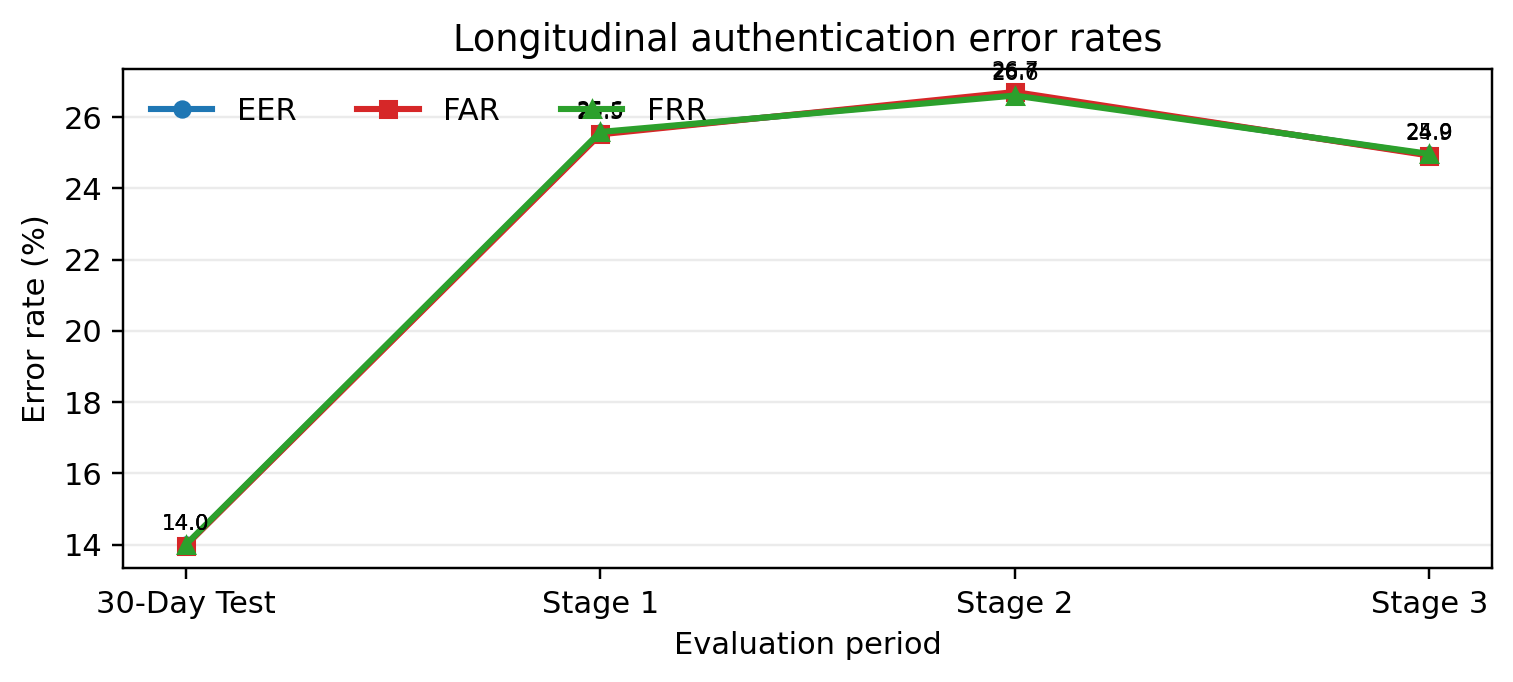
\includegraphics[width=\columnwidth]{longitudinal_drift_metrics.png}%
}{%
\fbox{\parbox{0.92\columnwidth}{\centering Generate this figure with \texttt{python make\_drift\_metrics\_figure.py} before submission.}}%
}
\caption{EER, FAR, and FRR across the 30-day baseline and later evaluation stages. Rising error rates after enrollment provide the direct visualization of longitudinal drift. Values are generated from the saved longitudinal evaluation metrics.}
\label{fig:drift-metrics}
\end{figure}

For each period, EER is obtained by sweeping the decision threshold over the saved genuine and impostor scores and selecting the operating point where FAR and FRR are closest; FAR and FRR in Fig.~\ref{fig:drift-metrics} are reported at the fixed enrollment threshold. Thus, EER summarizes separability while the fixed-threshold FAR/FRR values quantify deployment risk. Later-stage EER values must be read from the committed longitudinal metrics artifact and are not inferred from the fixed-threshold rates.

To investigate the mechanism behind the drift, causal tracing uses the same normalized timing-feature sequence representation as the baseline. A clean first-30-day sequence is compared with a later-stage sequence, and hidden states are restored one layer at a time while measuring the change in the authentication score. The causal effect of a component is its score recovery relative to the corrupted/reference run; layers and components are ranked by absolute recovery. This identifies where the later-stage representation loses the baseline decision signal and ties the intervention analysis to the actual authentication output.

ROME is evaluated as a targeted rank-one update at the highest-ranked traced component. The key is the hidden representation at the intervention site, and the value is chosen so that the later-stage activation moves the authentication score toward the desired genuine-user direction. The edit is applied once and evaluated on held-out Stages~1--3. Post-edit EER, FAR, and FRR are measured using the unchanged threshold protocol, together with a retention check on first-30-day sequences. An edit is considered useful only if it reduces later-stage error without materially changing the enrollment-period operating point.

\begin{table}[t]
\centering
\caption{Longitudinal error rates used to establish drift. Adaptation before/after values are read from the saved causal-tracing/ROME evaluation artifact.}
\label{tab:longitudinal-drift}
\scriptsize
\begin{tabular}{lcccccc}
\toprule
Period & EER & FAR count & FAR & FRR count & FRR\\
\midrule
30-day test & saved artifact & 4,717/33,768 & 14.0\% & 1,171/8,368 & 14.0\%\\
Stage 1 & saved artifact & 381,718/1,496,000 & 25.5\% & 4,349/17,000 & 25.6\%\\
Stage 2 & saved artifact & 281,588/1,054,504 & 26.7\% & 3,188/11,983 & 26.6\%\\
Stage 3 & saved artifact & 178,577/716,584 & 24.9\% & 2,033/8,143 & 25.0\%\\
\bottomrule
\end{tabular}
\end{table}

The repository script \texttt{make\_drift\_metrics\_figure.py} generates Fig.~\ref{fig:drift-metrics} from the saved longitudinal metrics file. The same artifact should contain the causal-tracing/ROME before/after EER, FAR, FRR, and enrollment-retention results; this keeps the adaptation claim reproducible and prevents qualitative preliminary results from being mistaken for a measured improvement.

\fi
\end{document}
